\section{Section}

Here we share our experiences and insights, hoping to provide a guide for others facing similar challenges as we encountered recently while preparing revised manuscripts for prominent conferences and journals.
Many of the conferences and journals such as OOPSLA, PLDI, POPL, FSE, ICSE, and UIST etc. require revised manuscript submissions along with a clear diff to facilitate easy tracking of changes. 
Recently, as we navigated the revision process for our submissions, we observed a shared struggle within the research community. 
Like most people in Computer Science research, we use LaTex and we tried to use \ls{latexdiff}~\cite{latex-diff} to show modifications for our revisions. 
Initially, we faced several issues which were gut-wrenching on the final day of revision submission. It took us to try several available options, and finally, we figured out the correct options to generate a diff PDF to track the changes.


\subsection{Subsection}

Lorem ipsum dolor sit amet, consectetur adipiscing elit~\cite{veytsmanlatex}.
Sed aliquam nisl turpis, sit amet mollis leo accumsan vel.
Donec semper turpis dui, a porttitor lorem tincidunt id.
Phasellus gravida, purus non faucibus euismod, lectus tortor maximus elit, vestibulum lobortis purus turpis non urna.
Fusce feugiat lectus ut massa molestie, non interdum augue porta.
Nunc dapibus odio nec neque cursus, ut lacinia velit rutrum.
Duis tempor nulla velit, sed pellentesque nunc imperdiet ut.
Phasellus eget hendrerit neque.
Suspendisse aliquet nulla id sem aliquam aliquam sed a orci.
Duis sem est, hendrerit nec porttitor sit amet, maximus sed nulla.
Suspendisse et dictum massa.
Morbi non diam nec orci sodales eleifend.
Etiam eget finibus purus, a malesuada ipsum.
Nullam ac nisi nec elit faucibus aliquet.
Nulla feugiat velit sed sodales eleifend.
Donec orci nulla, viverra et mi in, sagittis egestas urna.

\begin{figure}[htbp]
  \centering
  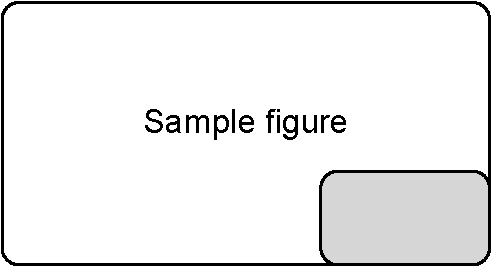
\includegraphics[scale=0.5]{sample-figure}
  \caption{Sample figure}
  \label{fig:sample}
\end{figure}

\subsubsection{Subsubsection}

This is a different \ls{onTouch()} in revision, Integer eleifend quam et odio iaculis, at elementum augue aliquam.
Ut eu nibh nec urna finibus semper fermentum id purus.
Aliquam eu sollicitudin libero.
Cras viverra elit congue erat pulvinar, vitae vehicula tortor interdum.
Aliquam commodo mi sapien, ullamcorper egestas velit tempor nec.
Quisque sapien velit, fringilla non vulputate nec, lacinia in dui.
Nam vestibulum volutpat ante, eu sodales enim tincidunt vel.
Ut mollis elit quis bibendum eleifend.
In laoreet tortor non odio ultrices mollis.
Curabitur volutpat et risus quis fermentum.
Morbi laoreet ligula eget orci consectetur, in dictum ipsum efficitur.
Mauris nec neque ultricies, efficitur elit id, hendrerit nibh.
Interdum et malesuada fames ac ante ipsum primis in faucibus.



\paragraph{Paragraph}

Nulla scelerisque id lectus a luctus.
Curabitur quis dolor maximus, maximus erat ut, placerat justo.
Donec auctor purus a lacus molestie maximus.
Etiam porta ligula a quam mollis efficitur.
Quisque vel sapien iaculis, pellentesque lorem nec, hendrerit lectus.
Vestibulum egestas congue euismod.
Praesent a tristique massa.
Aliquam eget ante elit.
Phasellus eget metus mi.
Fusce nec rutrum mi.
Pellentesque eu congue mi.
Fusce eu ullamcorper est.
